\noindent

\includegraphics[height=1.25cm]{images/pictograms/replication}
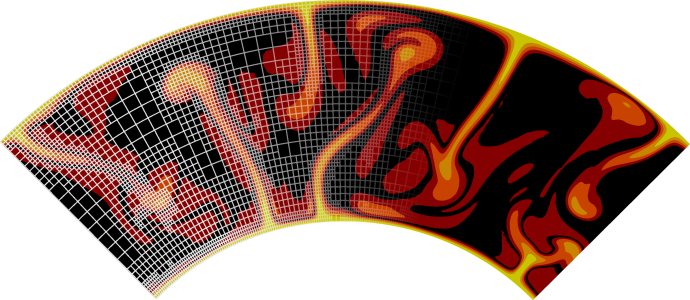
\includegraphics[height=1.25cm]{images/pictograms/aspect_logo}

\includegraphics[height=1.25cm]{images/pictograms/benchmark}

\includegraphics[height=1.25cm]{images/pictograms/under_construction}

\includegraphics[height=1.25cm]{images/pictograms/FEM}

\includegraphics[height=1.25cm]{images/pictograms/paraview}

%%%%%%%%%%%%%%%%%%%%%%%%%%%%%%%%%%%%%%%%%%%%%%%%%%%%%%%%%%%%%%%%%%%%%%%%%%%%%%%%%%%%%%%%%%%%%%%%%%%

\begin{flushright} {\tiny {\color{gray} \tt python\_codes/fieldstone\_160/text.tex}} \end{flushright}

%\lstinputlisting[language=bash,basicstyle=\small]{python_codes/template_keywords.key}

\par\noindent\rule{\textwidth}{0.4pt}

\begin{center}
\inpython
{\small Code: \url{https://github.com/cedrict/fieldstone/tree/master/python_codes/fieldstone_160}}
\end{center}

\par\noindent\rule{\textwidth}{0.4pt}

{\sl This stone was developed in collaboration with J.C. Afonso and C. Conrad}. 
\index{contributors}{J.C. Afonso}
\index{contributors}{C. Conrad}

\par\noindent\rule{\textwidth}{0.4pt}


%%%%%%%%%%%%%%%%%%%%%%%%%%%%%%%%%%%%%%%%%%%%%%%%%%%%%%%%%%%%%%%%%%%%%%%%%%%%%%%%%%%%%%%%%%%%%%%%%%%

%=========================================
\section*{Analytical exercise}

What follows is inspired by an experiment from an unpublished paper provided by J.C.

The domain is a Cartesian box of size $L_x=120~\si{\km}$, $L_y=120~\si{\km}$.
There are four materials in the domain:
\begin{itemize}
\item crust: $\rho_{c}=2300~\si{\kg\per\cubic\meter}$ and $\eta_{c}=10^{23}~\si{\pascal\second}$;
\item mantle: $\rho_{m}=3300~\si{\kg\per\cubic\meter}$ and $\eta_{m}=10^{21}~\si{\pascal\second}$;
\item weak zones: $\rho_{wz}=\rho_{c}$ and $\eta_{wz}=10^{-3}\eta_{c}$.
\item air or water: $\rho_a=0$ and $\eta_a << \eta_m$
\end{itemize}

The crust is 20~\si{\km} thick but is thickened (40~\si{\km} depth) in the middle 30~\si{\km}.
On each side we find weak zones as thick as the crust and 1~\si{\km} wide. 
The air layer is also 20~\si{\km} thick.

%\begin{center}
%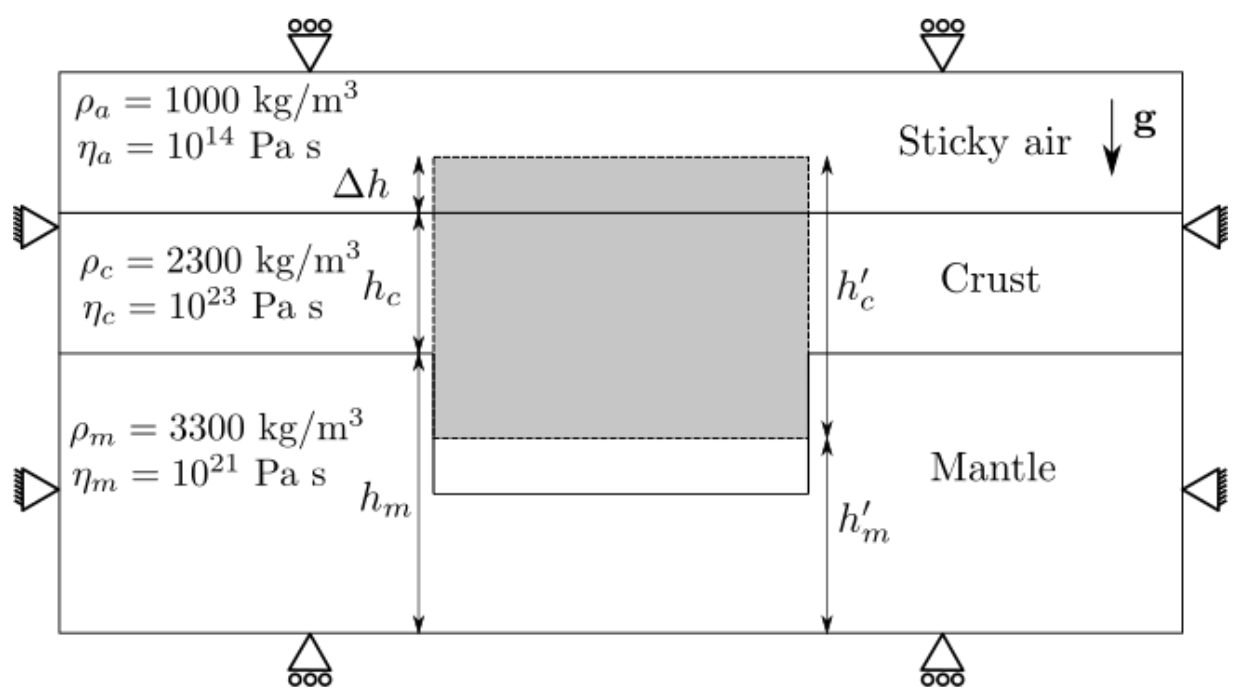
\includegraphics[width=9cm]{python_codes/fieldstone_160/images/setup}\\
%{\captionfont Figure by J.C. Afonso. $h_c$ and $h_m$ are the initial thicknesses of the crust and 
%mantle. $h_c'$ is the thickness of the thickened crust, and $h_m'$ is the thickness of the 
%mantle below the thickened crust at isostatic equilibrium. Drawing not to scale. The gray 
%area represents the final position of the tickened crust.}
%\end{center}

The thickened crust has a positive buoyancy with respect to the normal crust due
to density difference, whose analytical value is found via a standard isostatic balance (i.e.
equating the mass per unit area of two columns at the compensation level, here taken at
the base of the domain).

\newpage
\begin{center}
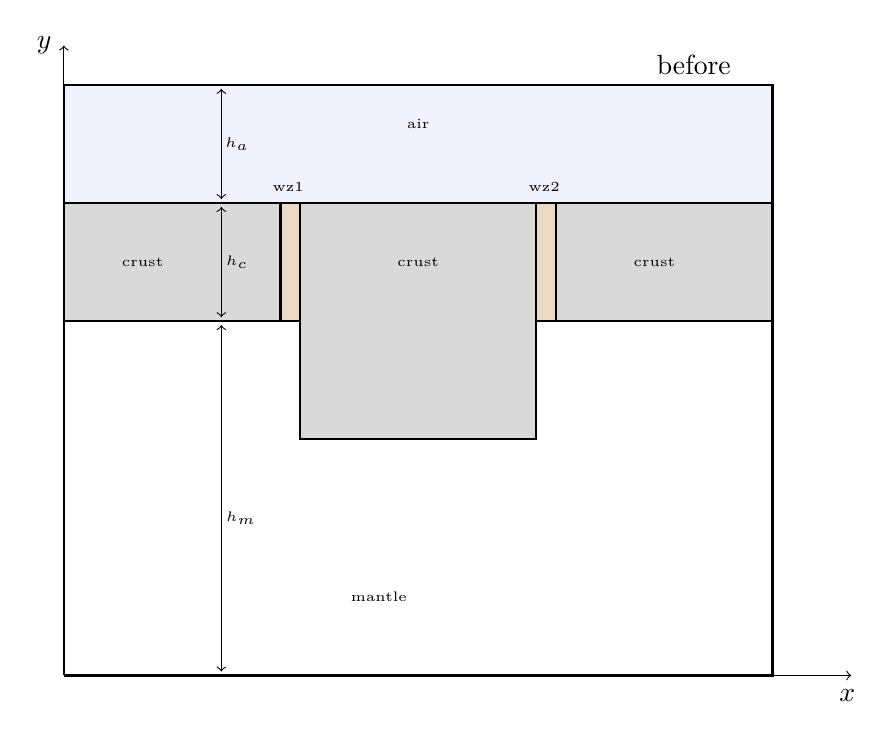
\begin{tikzpicture}
%\draw[fill=gray!23,gray!23](0,0) rectangle (11,8);
%\draw[step=0.5cm,gray,very thin] (0,0) grid (11,8); %background grid
\draw [fill=gray!30] (4,4) rectangle (7,7); 
\draw [fill=gray!30] (1,5.5) rectangle (3.75,7); 
\draw [fill=gray!30] (7.25,5.5) rectangle (10,7); 
\draw [fill=brown!30] (3.75,5.5) rectangle (4,7); %wz1
\draw [fill=brown!30] (7,5.5) rectangle (7.25,7); %wz2
\draw [fill=blue!5] (1,7) rectangle (10,8.5); %air
\draw[thick] (1,1) -- (10,1) -- (10,7) -- (1,7) --(1,1); 
\draw[thick] (1,5.5) -- (4,5.5) --(4,4)  --(7,4) --(7,5.5)--(10,5.5); 
\draw[thick] (3.75,5.5) -- (4,5.5) -- (4,7) -- (3.75,7) --(3.75,5.5); %weak zone left
\draw[thick] (7,5.5) -- (7.25,5.5) -- (7.25,7) --(7,7) -- (7,5.5);%weak zone right
\draw[thin,->] (1,1) -- (11,1); %x
\draw[thin,->] (1,1) -- (1,9); %y
\node[] at (10.95,0.75) {$x$};
\node[] at (0.75,9) {$y$};
\node[] at (3.85,7.2) {\tiny wz1};
\node[] at (7.1,7.2) {\tiny wz2};
\node[] at (2,6.25) {\tiny crust};
\node[] at (5.5,6.25) {\tiny crust};
\node[] at (8.5,6.25) {\tiny crust};
\draw[thin,<->] (3,5.55) -- (3,6.95); \node[] at (3.2,6.25) {\tiny $h_c$};
\draw[thin,<->] (3,1.05) -- (3,5.45); \node[] at (3.25,3) {\tiny $h_m$};
\draw[thin,<->] (3,7.05) -- (3,8.45); \node[] at (3.2,7.75) {\tiny $h_a$};
\node[] at (5.5,8) {\tiny air};
\node[] at (5,2) {\tiny mantle};
\draw[thick] (1,7) -- (1,8.5) -- (10,8.5) -- (10,7);
\node[] at (9,8.75) {before};
\end{tikzpicture}

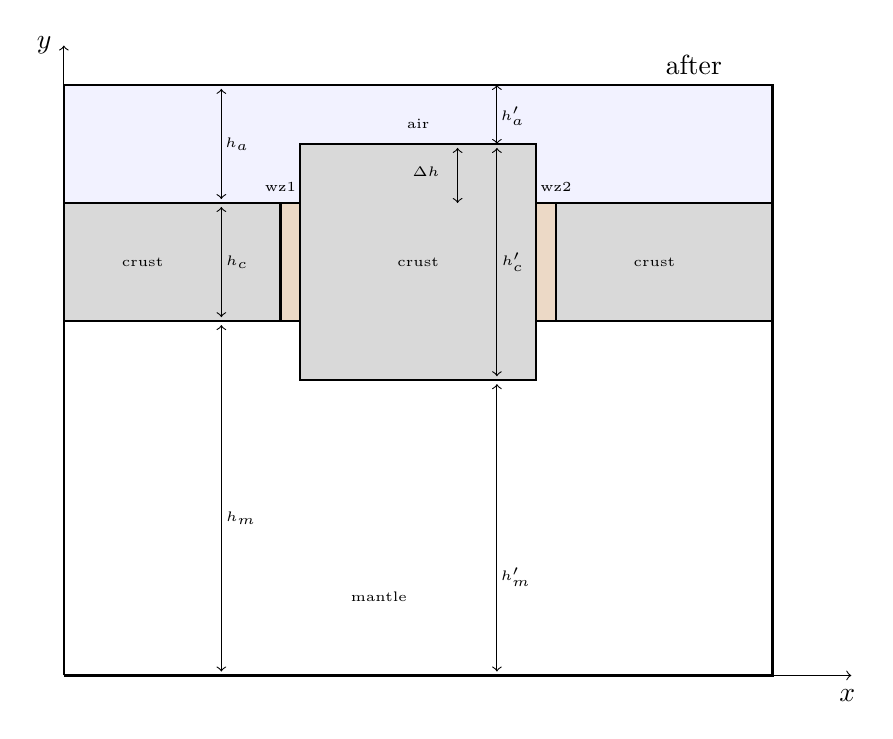
\begin{tikzpicture}
%\draw[fill=gray!23,gray!23](0,0) rectangle (11,8);
%\draw[step=0.5cm,gray,very thin] (0,0) grid (11,8); %background grid
\draw [fill=gray!30] (1,5.5) rectangle (3.75,7); 
\draw [fill=gray!30] (7.25,5.5) rectangle (10,7); 
\draw [fill=brown!30] (3.75,5.5) rectangle (4,7); %wz1
\draw [fill=brown!30] (7,5.5) rectangle (7.25,7); %wz2
\draw [fill=blue!5] (1,7) rectangle (10,8.5); %air
\draw [fill=gray!30] (4,4.75) rectangle (7,7.75); %middle crust
\draw[thick] (1,1)--(10,1)--(10,7)--(7,7)--(7,7.75)--(4,7.75)--(4,7)--(1,7) --(1,1); 
\draw[thick] (1,5.5) -- (4,5.5) --(4,4.75)  --(7,4.75) --(7,5.5)--(10,5.5); 
\draw[thick] (3.75,5.5) -- (4,5.5) -- (4,7) -- (3.75,7) --(3.75,5.5); %weak zone left
\draw[thick] (7,5.5) -- (7.25,5.5) -- (7.25,7) --(7,7) -- (7,5.5);%weak zone right
\draw[thin,->] (1,1) -- (11,1); %x
\draw[thin,->] (1,1) -- (1,9); %y
\node[] at (10.95,0.75) {$x$};
\node[] at (0.75,9) {$y$};
\node[] at (3.75,7.2) {\tiny wz1};
\node[] at (7.25,7.2) {\tiny wz2};
\node[] at (2,6.25) {\tiny crust};
\node[] at (5.5,6.25) {\tiny crust};
\node[] at (8.5,6.25) {\tiny crust};
\draw[thin,<->] (3,5.55) -- (3,6.95); \node[] at (3.2,6.25) {\tiny $h_c$};
\draw[thin,<->] (3,1.05) -- (3,5.45); \node[] at (3.25,3) {\tiny $h_m$};
\draw[thin,<->] (3,7.05) -- (3,8.45); \node[] at (3.2,7.75) {\tiny $h_a$};
\node[] at (5.5,8) {\tiny air};
\node[] at (5,2) {\tiny mantle};
\draw[thick] (1,7) -- (1,8.5) -- (10,8.5) -- (10,7); %top line of domain aove air
\draw[thin,<->] (6.5,7.75) -- (6.5,8.5); \node[] at (6.7,8.1) {\tiny $h_a'$};
\draw[thin,<->] (6.5,4.8) -- (6.5,7.7); \node[] at (6.7,6.25) {\tiny $h_c'$};
\draw[thin,<->] (6.5,1.05) -- (6.5,4.7); \node[] at (6.74,2.25) {\tiny $h_m'$};
\node[] at (9,8.75) {after};

\draw[thin,<->] (6,7) -- (6,7.7); \node[] at (5.6,7.4) {\tiny $\Delta h$};

\end{tikzpicture}

{\captionfont $h_c$ and $h_m$ are the initial thicknesses of the crust and 
mantle. $h_c'$ is the thickness of the thickened crust, and $h_m'$ is the thickness of the 
mantle below the thickened crust at isostatic equilibrium. Drawing not to scale. 
wz1 and wz2 stand for 'weak zone' 1 \& 2.}
\end{center}

Note that these drawings are very conceptual: for example one would expect the weak zones
to deform while the thickned crust is moving up. Also, between the two figures mantle volume 
and air volume are not conserved.

Clint commented: 
\begin{displayquote}
{\color{darkgray}
I would call this isostatic topography, not dynamic topography. The definition 
of dynamic topography is debated, but generally the debate is whether temperature-induced variations 
in density within the mantle lithosphere should be called dynamic topography or isostatic topography. 
I think pretty much universally crustal variations are referred to isostatic topography - 
so calling this dynamic topography here might be confusing to some. 
But I can see where you are coming from and this is an interesting and illustrative test. 
I would just suggest adding a note that this topography is well-understood, and it is usually considered isostatic topography.
}
\end{displayquote}

In lecture notes by S. Zhong, I found:
\begin{displayquote}
{\color{darkgray}
Dynamic topography is that due to non-isostatic (i.e.,
non-crustal and non-lithospheric) effects, i.e.,
residual topography after correcting for isostatic
effects or crustal and lithospheric contributions to
the topography.

Dynamic topography is important because it tells us
about the dynamics. It is also more difficult to get
because some tricky ``corrections'' are needed.
}
\end{displayquote}




\newpage


%-----------------------------
\subsection*{Air layer case}

Let us now assume $\rho_a=0$. 

On the left or right sides (i.e. $x=0$ or $x=L_x$), the lithostatic pressure at the base of the crust is then 
$\rho_{c} g h_{c}=2300 \cdot 10 \cdot20000=460~\si{\mega\pascal}$.
At the base of the model, then the pressure is $460e6+\rho_{m} g h_{m}
=460e6+3300 \cdot 10 \cdot 80000=460e6+2640e6=3100~\si{\mega\pascal}$.
In a more abstract way, $P_{bottom}=\rho_c g h_c + \rho_m g h_m$.

In the middle, after the block has moved up and is now in isostatic equilibrium, 
we should have $P_{bottom}=\rho_c g h_c' + \rho_m g h_m'$.
In the end:
\[
P_{bottom}=\rho_c g h_c + \rho_m g h_m = \rho_c g h_c' + \rho_m g h_m'
\]
We can divide both sides by $g$:
\begin{eqnarray}
\rho_c  h_c + \rho_m  h_m &=& \rho_c  h_c' + \rho_m  h_m' \nn\\
\Rightarrow \rho_m h_m'&=& \rho_c(h_c-h_c') + \rho_m h_m  \nn\\
\Rightarrow h_m' &=& h_m-(h_c'-h_c)\frac{\rho_c}{\rho_m} \nn
\end{eqnarray}
Then the dynamic topography is computed as follows:
\begin{eqnarray}
\Delta h 
&=& h_c' + h_m' - h_c - h_m \nn\\
&=& h_c' + h_m -(h_c'-h_c)\frac{\rho_c}{\rho_m} -h_c - h_m \nn\\
&=& h_c'  -(h_c'-h_c)\frac{\rho_c}{\rho_m} -h_c  \nn\\
&=& (h_c'-h_c)  -(h_c'-h_c)\frac{\rho_c}{\rho_m}   \nn\\
&=& (h_c'-h_c) \left(1 -\frac{\rho_c}{\rho_m} \right) 
\end{eqnarray}
Substituting for the parameters of our example, the predicted topography uplift is 
\[
\Delta h = (40000-20000)\cdot (1-2300/3300) \simeq 6060~\si{\meter}
\]


%-----------------------------
\subsection*{Water layer case}

In this case we set $\rho_a=1000$.

On the left side we have $P_{bottom}=\rho_a g h_a + \rho_c g h_c + \rho_m g h_m$, which 
yields $P_{bottom}=(1000*20e3 + 2300*20e3 + 3300*80e3)*10 = 33e8=3300~\si{\mega\pascal}$.
In the middle:
$P_{bottom}=\rho_a g h_a' + \rho_c g h_c' + \rho_m g h_m'$.

\begin{eqnarray}
P_{bottom}
&=&\rho_a g h_a + \rho_c g h_c + \rho_m g h_m \nn\\
&=& \rho_a g h_a' + \rho_c g h_c' + \rho_m g h_m' \nn
\end{eqnarray}
or, after diving by $g$:
\begin{eqnarray}
\rho_a  h_a + \rho_c  h_c + \rho_m  h_m
&=& \rho_a  (h_a-\Delta h) + \rho_c  h_c' + \rho_m  h_m' \nn 
\end{eqnarray}
which we write:
\begin{eqnarray}
\rho_m  h_m' 
&=&  \rho_a  h_a + \rho_c  h_c + \rho_m  h_m - [\rho_a  (h_a-\Delta h) + \rho_c  h_c'] \nn\\
&=&  \rho_a  h_a + \rho_c  h_c + \rho_m  h_m - \rho_a  (h_a-\Delta h) - \rho_c  h_c' \nn\\
&=&  \rho_c  h_c + \rho_m  h_m + \rho_a  \Delta h - \rho_c  h_c' 
\end{eqnarray}
Looking at the figure we also have 
\begin{eqnarray}
\Delta h 
&=& h_c' + h_m' - h_c - h_m \nn\\
&=& h_c' + \frac{1}{\rho_m}[\rho_c  h_c + \rho_m  h_m + \rho_a  \Delta h - \rho_c  h_c'] - h_c - h_m \nn\\
&=& h_c' + \frac{\rho_c}{\rho_m} h_c +  h_m + \frac{\rho_a}{\rho_m} \Delta h - \frac{\rho_c}{\rho_m} h_c' - h_c - h_m \nn\\
&=& h_c' + \frac{\rho_c}{\rho_m} h_c + \frac{\rho_a}{\rho_m} \Delta h - \frac{\rho_c}{\rho_m} h_c' - h_c \nn\\
(1 - \frac{\rho_a}{\rho_m})\Delta h &=& h_c' + \frac{\rho_c}{\rho_m} h_c - \frac{\rho_c}{\rho_m} h_c' - h_c \nn\\
(1 - \frac{\rho_a}{\rho_m})\Delta h &=& (1 - \frac{\rho_c}{\rho_m})h_c' -(1 - \frac{\rho_c}{\rho_m}) h_c \nn\\
(1 - \frac{\rho_a}{\rho_m})\Delta h &=& (1 - \frac{\rho_c}{\rho_m})(h_c' - h_c) \nn\\
\Delta h &=&(1 - \frac{\rho_a}{\rho_m})^{-1}  (1 - \frac{\rho_c}{\rho_m})(h_c' - h_c) \nn\\
\Delta h &=& \frac{\rho_m}{\rho_m-\rho_a}  \frac{\rho_m-\rho_c}{\rho_m} (h_c' - h_c) \nn\\
\Delta h &=&  \frac{\rho_m-\rho_c}{\rho_m-\rho_a} (h_c' - h_c) 
\end{eqnarray}

In this case we get 
\[
\Delta h =  \frac{ 3300- 2300}{3300-1000} (40e3 - 20e3) = \frac{1000}{2300} 20e3 \simeq 8695~\si{\meter} 
\]
Obviously if we set $\rho_a=0$ we find the value obtained for air.

%-----------------------------
\subsection*{Clint's comments}

{\color{darkgray} Your predicted topography is basically isostatic topography: 
I get the same 6.06 km when I compute Airy topography using the equations from my Geodynamics notes}:

\begin{center}
\fbox{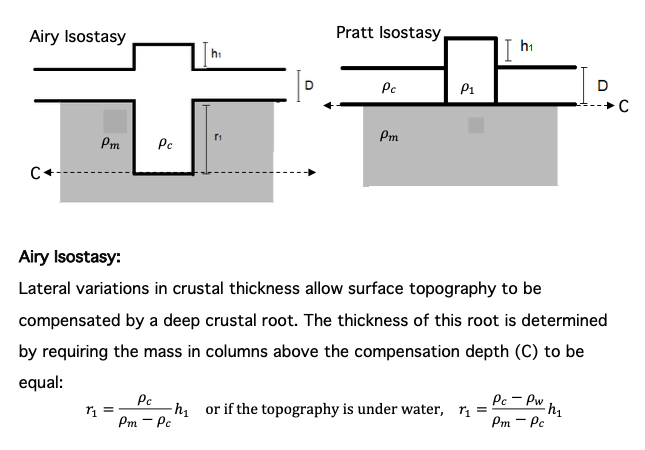
\includegraphics[width=8cm]{python_codes/fieldstone_160/images/img.png}}
\end{center}

{\color{darkgray}
However, this is topography above the surrounding topography - $h_1$ in the left figure.
I got this by considering that the topography is under water in this case, and $r_1+h_1=20$ km, 
then I use the right hand equation to find:
\[
20 km - h_1 = (\rho_c - \rho_w)/(\rho_m - \rho_c) *h_1
\]
\[
20 km = h_1 + (1300/1000) * h_1 = 2.3*h_1
\]
\[
h_1 = 8.69 km
\]
}








%===================================================
\section*{How to compute DT in geodynamical codes?}

\noindent In the \aspect manual we find the following documentation for the 'dynamic topography' post-processor:
\begin{displayquote}
{\color{darkgray}
A postprocessor that computes a measure of dynamic topography based on the stress at the boundary. 
The exact approach works as follows: At each selected boundary, we compute the traction that acts normal to 
the boundary faces using the consistent boundary flux method as described in \textcite{grls87} (1987).
From this traction, the dynamic topography is computed using the formula $h=\sigma_n / \rho g$ where $g$
is the norm of the gravity and $\rho$
is the density [of the fluid right below the surface]. 
}
\end{displayquote}

\noindent 
In practice the dynamic topography is then computed as follows: 
\[
h= \frac{\vec{n} \cdot {\bm \sigma}\cdot \vec{n}}{\rho_c g } 
= \frac{\sigma_{yy}}{\rho_c g}
= \frac{-p+\tau_{yy}}{\rho_c g}
\]
where $\vec{n}$ is the normal vector to the surface\footnote{$\vec{t} ={\bm\sigma}\cdot \vec{n}$ 
is the traction on the boundary and then $\vec n \cdot \vec t$ is the component of this traction
along the normal.}. 

Clint adds:
\begin{displayquote}
{\color{darkgray}
We usually use the full normal stress $\sigma_n$ to compute dynamic topography as $h=\sigma_n/(\delta \rho * g)$
It is important to keep the pressure term (and not omit it as with deviatoric stress) because pressure variations 
also contribute to dynamic topography. The idea is that if the boundary cannot move vertically (no free surface), 
then the stress on that boundary tells us what the topography *would be* if the surface could move. 
(I guess this can be tested with a code that can handle a free surface).
\\
Setting the surface average equal to zero would mean that the average dynamic topography $h$ 
is also zero (if $\delta \rho$ is constant) - we kind of used this in this paper (based on CitComS):
\textcite{cohu09} (2009).
The zero-average dynamic topography means that if dynamic topography on the continents is on-average 
increasing, then it is decreasing on-average over the oceans, leading to sea level drop.
\\
One interesting thing that we explored in our 2009 paper: Let’s say you have a dense blob 
in the mantle - it produces negative dynamic topography at the surface that gets smaller 
with time as the blob descends. Thus, the sense of motion is uplift. 
Now consider a low-density blob - this produces positive dynamic topography that gets 
bigger with time as the blob gets closer to the surface - also uplift! 
So you get uplift above both positive and negative density anomalies in 
the mantle. By the same logic, you would always get CMB subsidence below positive and negative 
density anomalies. But I guess you get the opposite behavior everywhere else 
away from above/below the density anomaly, so everything evens out. 

}
\end{displayquote}


\newpage
%=========================================================
\section*{Results}

Let us now investigate this by means of numerical modelling. 
For many decades (and still now for large 3D spherical models) 
so-called sticky-air, sticky-water or true free surface was not an option 
and people relied on free surface boundary conditions at the top of the 
crust, only to use the algorithm above to arrive at an estimate 
of the equivalent topography.


The setup/geometry for the calculations is as follows

\begin{center}
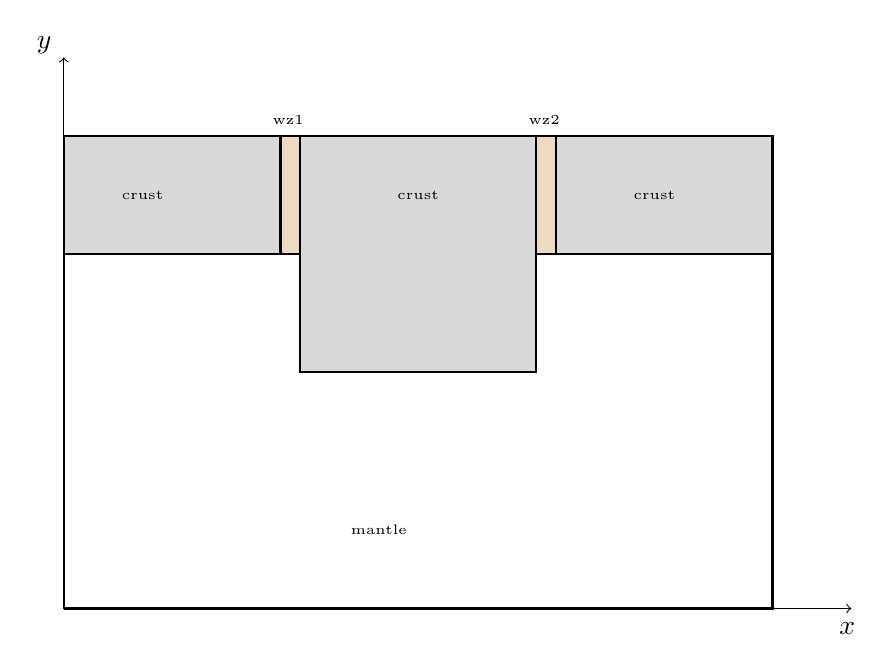
\begin{tikzpicture}
%\draw[fill=gray!23,gray!23](0,0) rectangle (11,8);
%\draw[step=0.5cm,gray,very thin] (0,0) grid (11,8); %background grid
\draw [fill=gray!30] (4,4) rectangle (7,7); 
\draw [fill=gray!30] (1,5.5) rectangle (3.75,7); 
\draw [fill=gray!30] (7.25,5.5) rectangle (10,7); 
\draw [fill=brown!30] (3.75,5.5) rectangle (4,7); %wz1
\draw [fill=brown!30] (7,5.5) rectangle (7.25,7); %wz2

\draw[thick] (1,1) -- (10,1) -- (10,7) -- (1,7) --(1,1); 
\draw[thick] (1,5.5) -- (4,5.5) --(4,4)  --(7,4) --(7,5.5)--(10,5.5); %8-6-2
\draw[thick] (3.75,5.5) -- (4,5.5) -- (4,7) -- (3.75,7) --(3.75,5.5); %weak zone left
\draw[thick] (7,5.5) -- (7.25,5.5) -- (7.25,7) --(7,7) -- (7,5.5);%weak zone right
\draw[thin,->] (1,1) -- (11,1); %x
\draw[thin,->] (1,1) -- (1,8); %y
\node[] at (10.95,0.75) {$x$};
\node[] at (0.75,8.15) {$y$};
\node[] at (3.85,7.2) {\tiny wz1};
\node[] at (7.1,7.2) {\tiny wz2};
\node[] at (2,6.25) {\tiny crust};
\node[] at (5.5,6.25) {\tiny crust};
\node[] at (8.5,6.25) {\tiny crust};
%\draw[thin,<->] (3,5.55) -- (3,6.95); \node[] at (3.2,6.25) {\tiny $h_c$};
%\draw[thin,<->] (3,1.05) -- (3,5.45); \node[] at (3.25,3) {\tiny $h_m$};
\node[] at (5,2) {\tiny mantle};
\end{tikzpicture}

{\captionfont Drawing not to scale.}
\end{center}

Free slip boundary conditions are imposed on all four sides.
To be very clear, the air/water layer is absent so that the domain is $120\times100~\si{\km}$.
 ${\bm Q}_2 \times Q_1$ (continuous pressure)
or ${\bm Q}_2\times P_{-1}$ (discontinuous pressure) elements are used.
The boundary conditions are such that the pressure can only be computed up to a constant (null space)
and it is therefore normalised by imposing that the average pressure at the surface is zero 
(the implicit assumption being that the air above it is massless).
Concerning this Clint states:
\begin{displayquote}
{\color{darkgray}
Removing the average pressure to me makes sense. If there were net positive pressure on the boundary, 
then we could think about this as a net shift of the entire boundary upwards, meaning that we could 
choose a slightly thicker box (or larger earth radius) to make the average pressure zero - in 
some sense this is an arbitrarily chosen parameter. I guess one challenging thing to think about would 
be how to handle changes in the pressure that develop over time - if this even happens in the models? 
I guess these would correspond to changes in volume that happen over time - for example based on changes 
in average temperature (heating or cooling earth). For an incompressible calculation this would not result 
in a change in volume, but for compressible convection I think it might be - a warming earth would be less 
dense, meaning that its radius should expand, resulting in dynamic topography that grows with time. But I 
think this component would be missed if the pressure is always removed from the stress at the surface. 
This paper discusses this, and seems to suggest (in the abstract) that the earth radius cannot change with 
time (even for compressible convection?) \cite{foro22}.
}
\end{displayquote}



In all what follows temperature effects are discarded. A single Stokes solve is carried out, without any 
time stepping nor advection of the materials.
The default resolution is set to 120$\times$100 elements.

\begin{center}
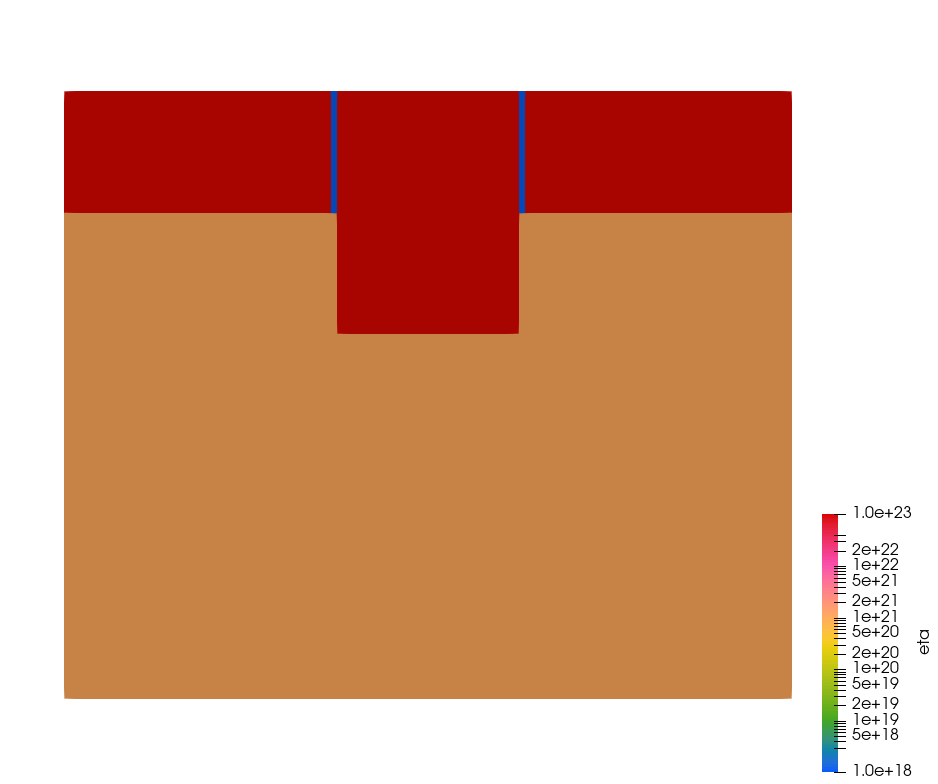
\includegraphics[width=8.5cm]{python_codes/fieldstone_160/results/eta.png}
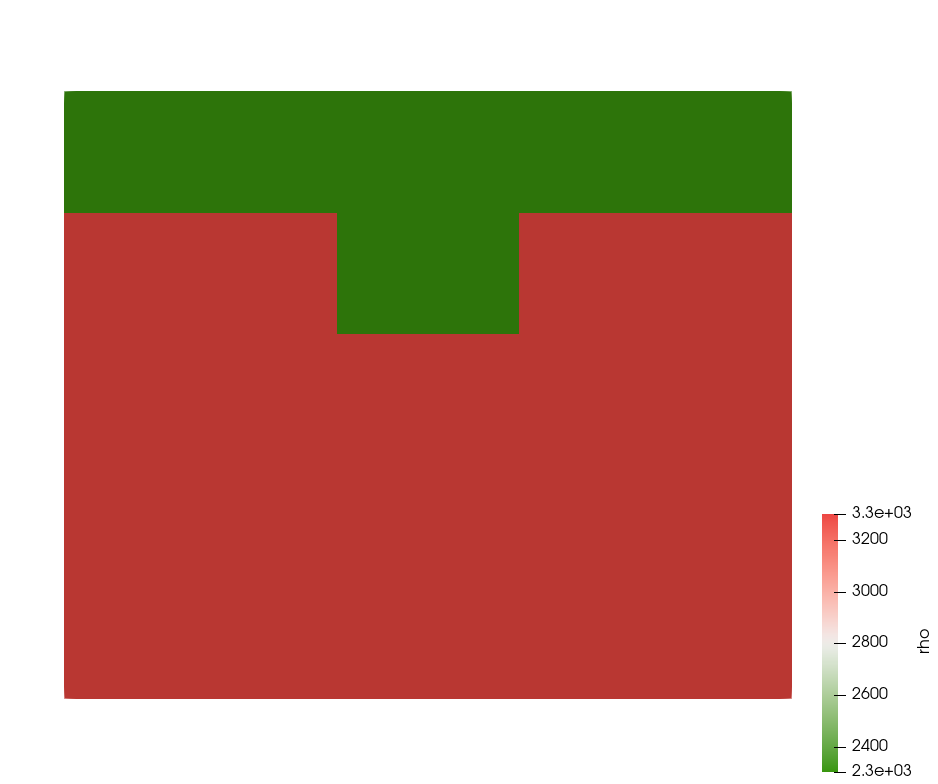
\includegraphics[width=8.5cm]{python_codes/fieldstone_160/results/rho.png}\\
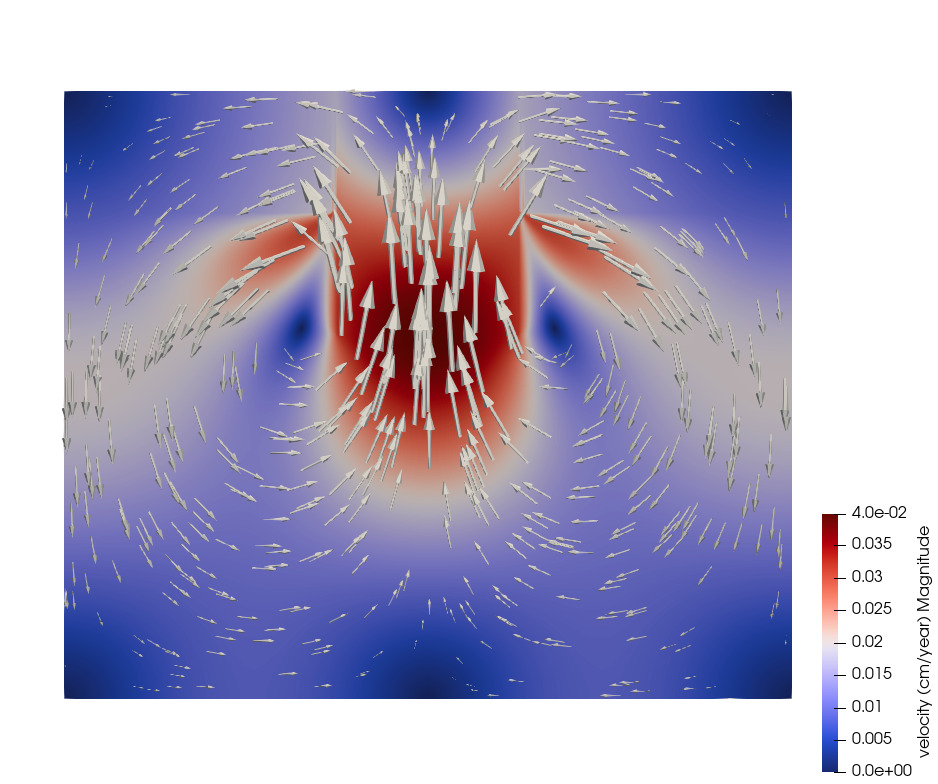
\includegraphics[width=8.5cm]{python_codes/fieldstone_160/results/vel.jpg}
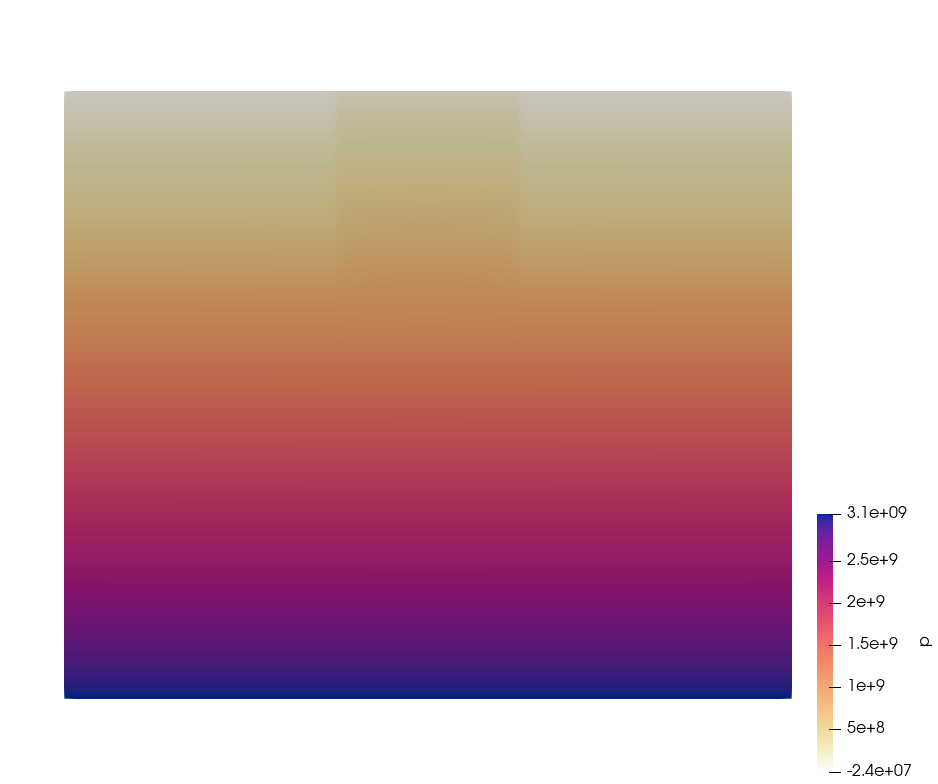
\includegraphics[width=8.5cm]{python_codes/fieldstone_160/results/press.png}\\
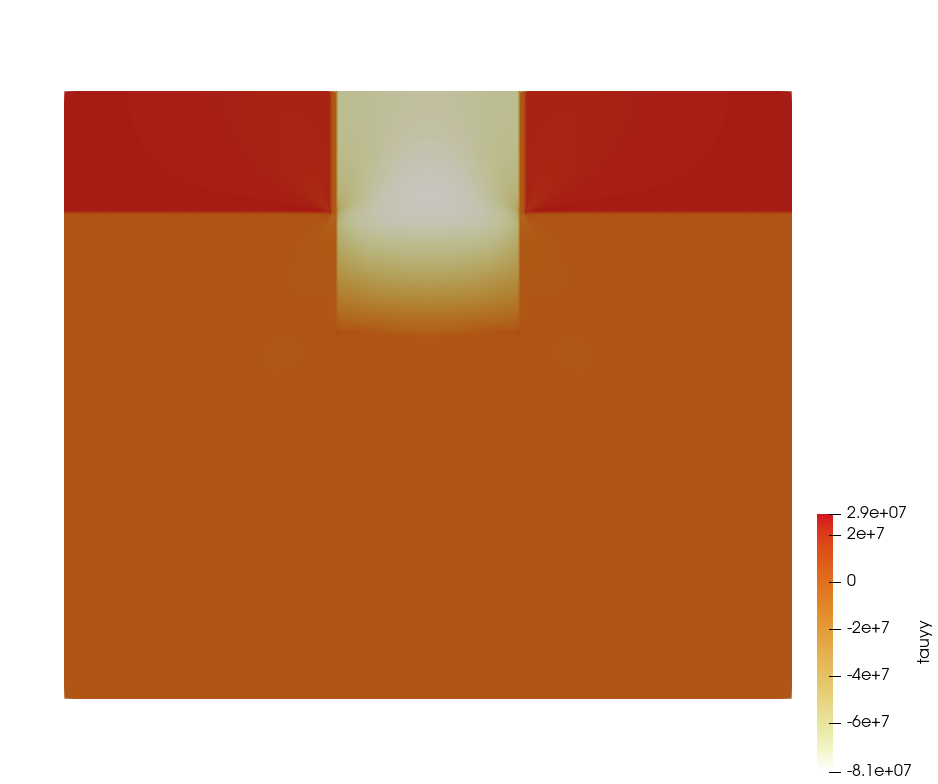
\includegraphics[width=8.5cm]{python_codes/fieldstone_160/results/tau_yy.png}
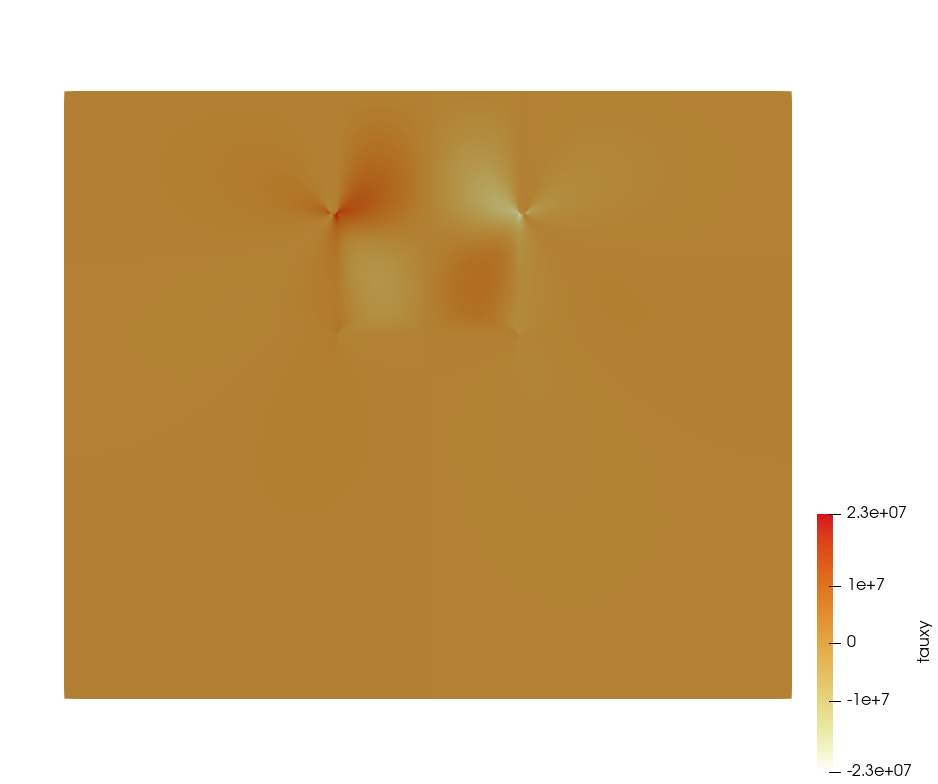
\includegraphics[width=8.5cm]{python_codes/fieldstone_160/results/tau_xy.png}\\
{\captionfont Results obtained on 240x200 mesh. Top row: viscosity and density fields;
Middle row: velocity and pressure fields; 
Bottom row: $\tau_{yy}$ and $\tau_{xy}$ fields.}
\end{center}


\newpage

\subsubsection*{Reference case}

The surface pressure, $yy$ component of deviatoric stress ${\bm \tau}$ 
and dynamic topography are shown in the following plots:
\begin{center}
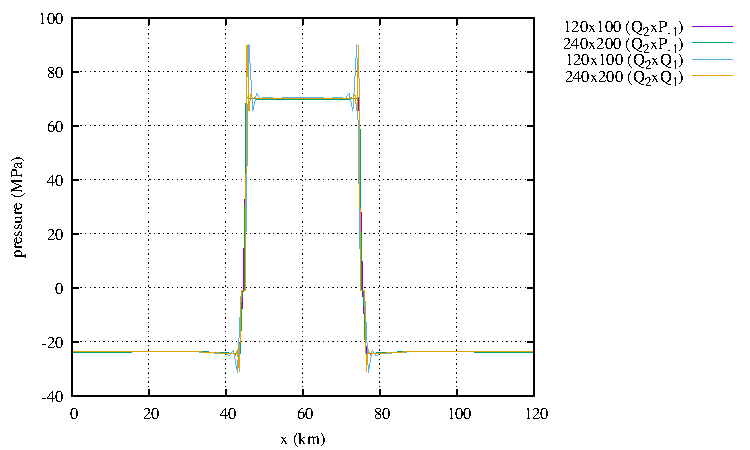
\includegraphics[width=8.5cm]{python_codes/fieldstone_160/results/pressure.pdf}
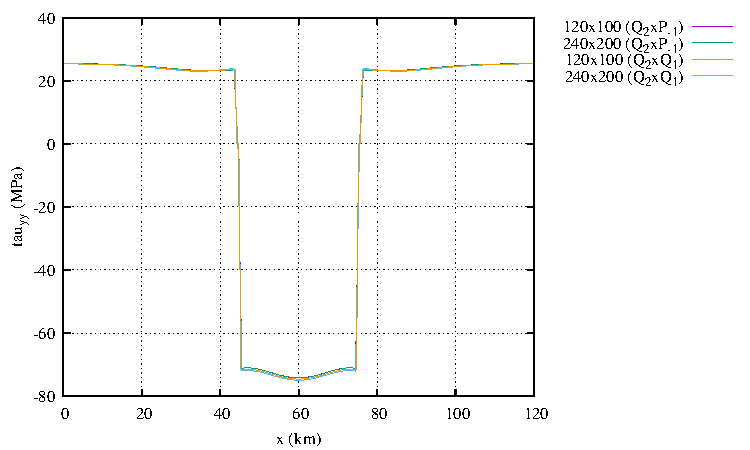
\includegraphics[width=8.5cm]{python_codes/fieldstone_160/results/tau_yy.pdf}\\
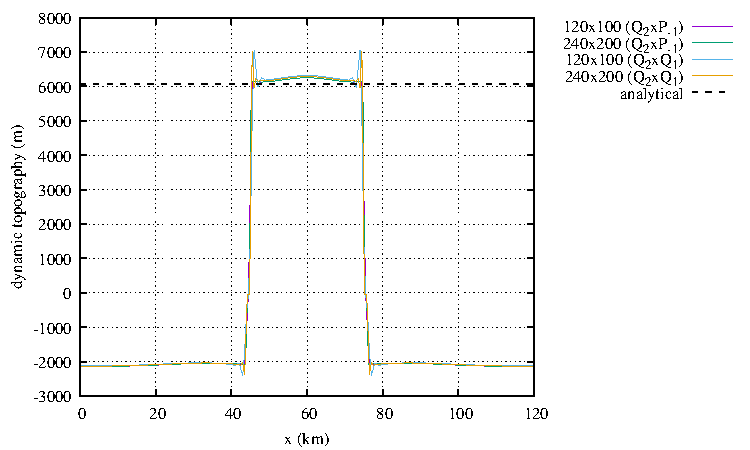
\includegraphics[width=8.5cm]{python_codes/fieldstone_160/results/dyn_topo.pdf}
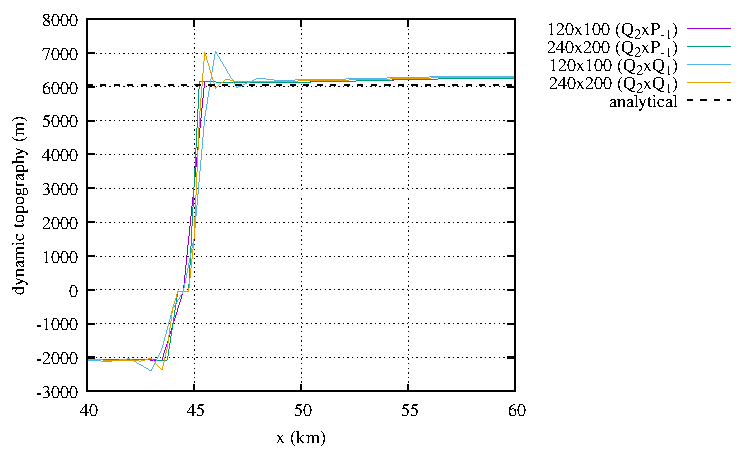
\includegraphics[width=8.5cm]{python_codes/fieldstone_160/results/dyn_topo2.pdf}
\end{center}
We find that the differences between low and high resolution are really small. 
The recovered dynamic topography is very close to the expected analytical value,
but since its accuracy is not improving with resolution this probably means that the 
weak zones and/or the coupling of the keel of the crust with the mantle is 
playing a prominent role.

We also find that the discontinuous pressure element unsurprisingly copes better 
with the element boundary-aligned viscosity jumps, while the continuous pressure 
one yields overshoots on the pressure field.

Note that the topography is about 6000~\si{\meter} relative to the zero, but since the 
crust left and right has a topography of about -2000~\si{\meter}, then the `real' 
topography is more akin to 8000~\si{\meter}.

\subsubsection*{Influence of the weak zones viscosity}

Let us now investigate the influence of the weak zones viscosity on the 
dynamic topography (zoomed on the important part in the right figure):
\begin{center}
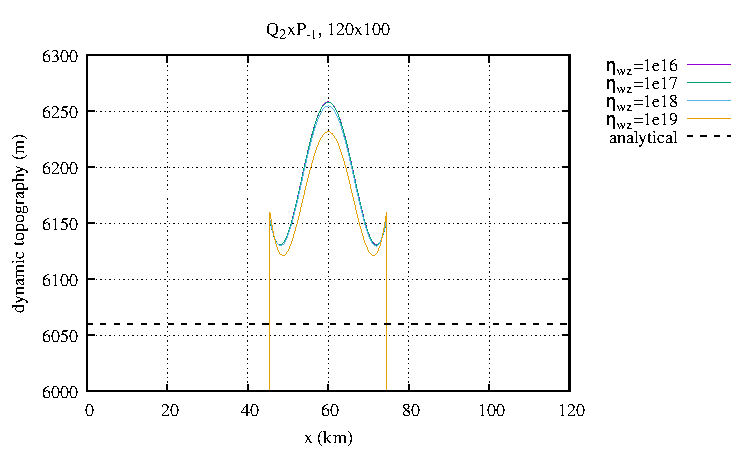
\includegraphics[width=8.5cm]{python_codes/fieldstone_160/results/dyn_topo3a.pdf}
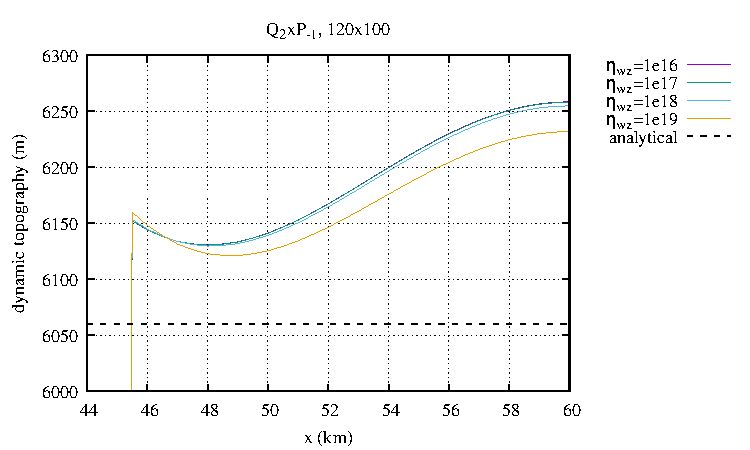
\includegraphics[width=8.5cm]{python_codes/fieldstone_160/results/dyn_topo3b.pdf}
\end{center}
The default value of $\eta_{wz}=10^{18}~\si{\pascal\second}$ is clearly low enough since lower values do not 
yield any meaningful change. This means that the signal we observe is entirely due
to the geometry of the experiment and/or the coupling crust keel-mantle.

\subsubsection*{Influence of the mantle viscosity}

We can now look at the influence of the mantle viscosity (while keeping the 
weak zones at $\eta_{wz}=10^{18}~\si{\pascal\second}$):
\begin{center}
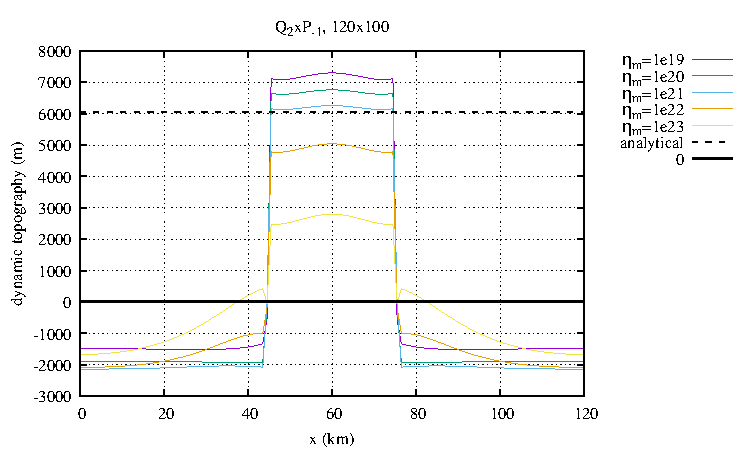
\includegraphics[width=8.5cm]{python_codes/fieldstone_160/results/dyn_topo4a.pdf}
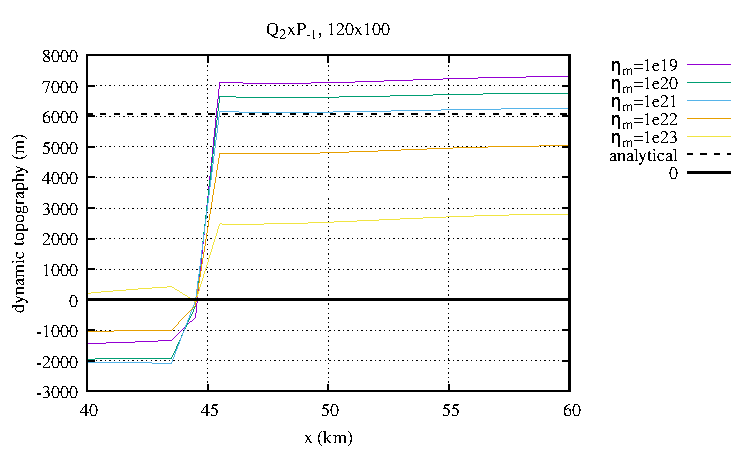
\includegraphics[width=8.5cm]{python_codes/fieldstone_160/results/dyn_topo4b.pdf}
\end{center}
The higher the viscosity of the mantle, the lower the dynamic topography. 
It appears that $\eta_m=10^{21}~\si{\pascal\second}$ yields a dynamic topography
closest to the expected theoretical value.
It is also worth noting that on each side of the block the dynamic topography
is about -2000m.
Looking at the velocity field on the previous page figure, we see that the domain
is such that the positive buoyancy of the block generates a convection cell which 
therefore pulls down the crust on each side of the block.

Clint comments:
\begin{displayquote}
{\color{darkgray}
In this figure you get increasingly smaller topography as you increase the mantle viscosity. 
I think what you are seeing here is only partially compensated topography (not yet in isostatic equilibrium) 
- kind of a GIA process that has not run to completion. The timescale for this to happen is longer for 
higher mantle viscosity, so the topography has relaxed less for the higher viscosity cases. 
For the 1e19 Pa s case (purple line), then it is actually almost fully compensated already. My prediction is 
that if you let these systems run for many timesteps then the region of thick crust would pop up more and more, 
until it reaches they all reach theoretical value of 8.69 km above the surrounding topography [if water was 
indeed present above the crust]. 
This might take a long time for the 1e23 Pa s case. The timescale for relaxation also depends on wavelength, 
so you could make these run faster if you make the thick crust region wider.
}
\end{displayquote}

%..............................................
\subsubsection*{Influence of the box geometry}

Let us now investigate the influence of the box geometry (and in particular its 
lateral extent $L_x$ while keeping a $1\times 1$ km resolution). 
\begin{center}
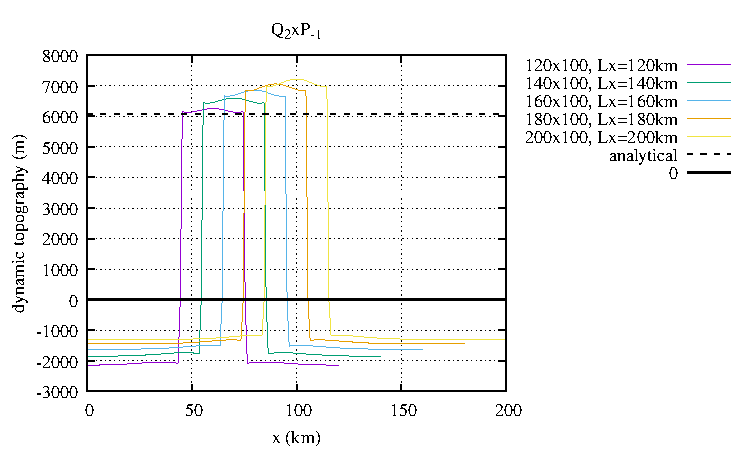
\includegraphics[width=8.5cm]{python_codes/fieldstone_160/results/dyn_topo5.pdf}
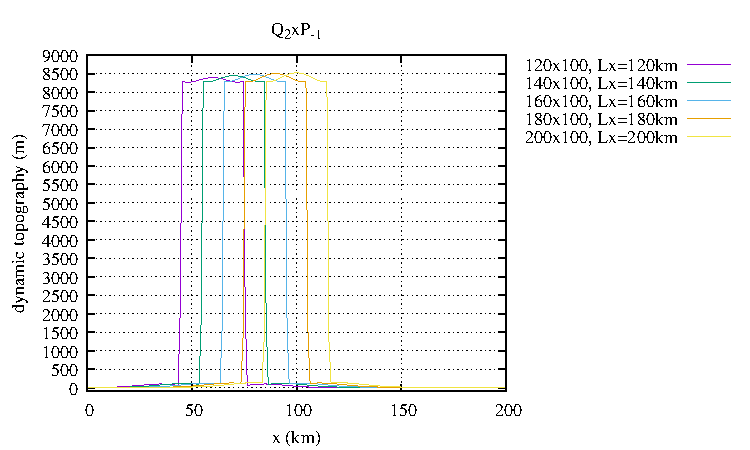
\includegraphics[width=8.5cm]{python_codes/fieldstone_160/results/dyn_topo5b.pdf}\\
{\captionfont Left: raw signal; Right: signal offset so that DT is zero on the 
sides of the domain.}
\end{center}
We find that the dynamic topography depends mildly on this parameter (all other
things equal), which is evident when the signals are offset so that the topograhy
is zero on the sides (right figure above).

In light of all this, let us now prescribe the lithostatic pressure (Neumann boundary conditions)
on the left and right boundaries so as to allow for free in/outflow and hopefully tame the 
return flow. A single node in the middle of the bottom boundary is assigned $u=0$ so as 
to remove the translational nullspace. We obtain the following velocity field 
for the default setup:
\begin{center}
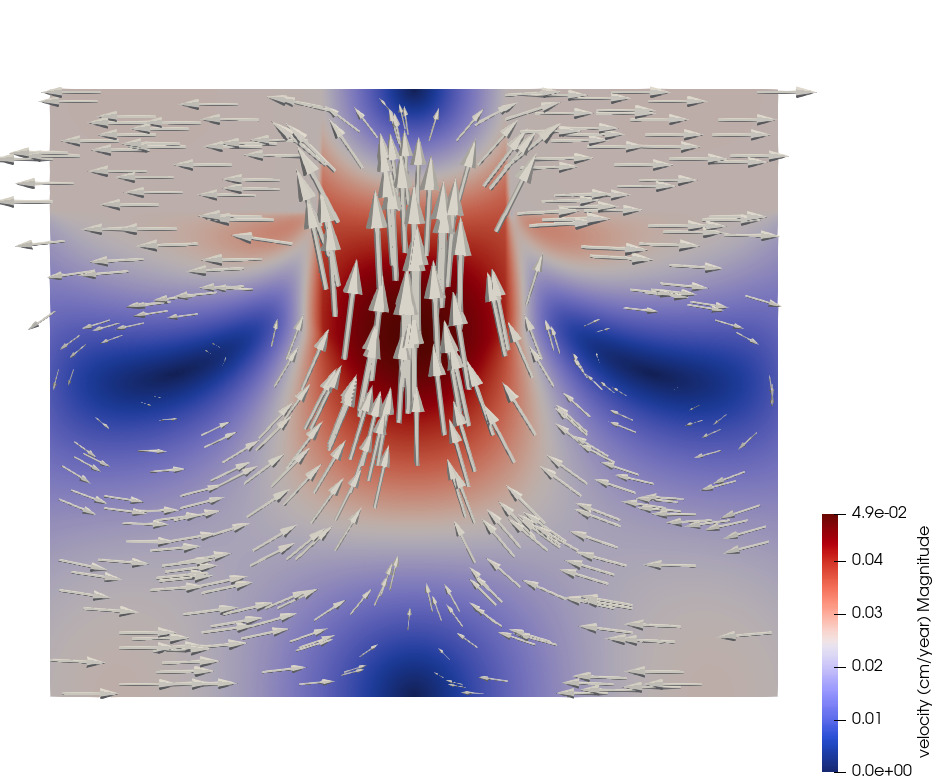
\includegraphics[width=8.5cm]{python_codes/fieldstone_160/results/neumann/velN}
\end{center}
and the dynamic topography varies with $L_x$ as follows:
\begin{center}
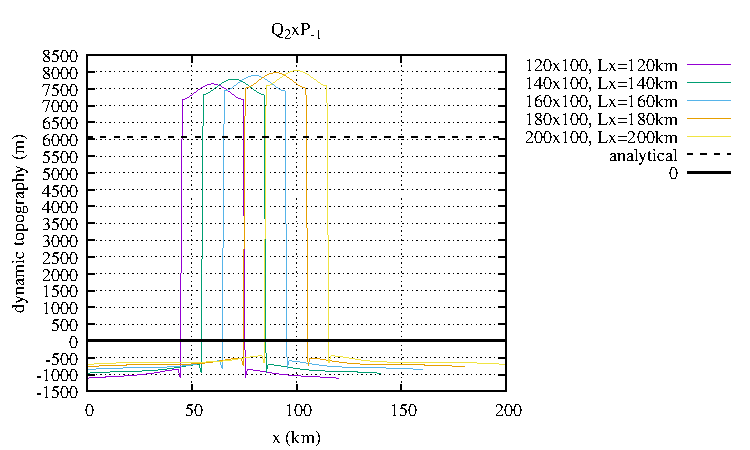
\includegraphics[width=8.5cm]{python_codes/fieldstone_160/results/dyn_topo6.pdf}
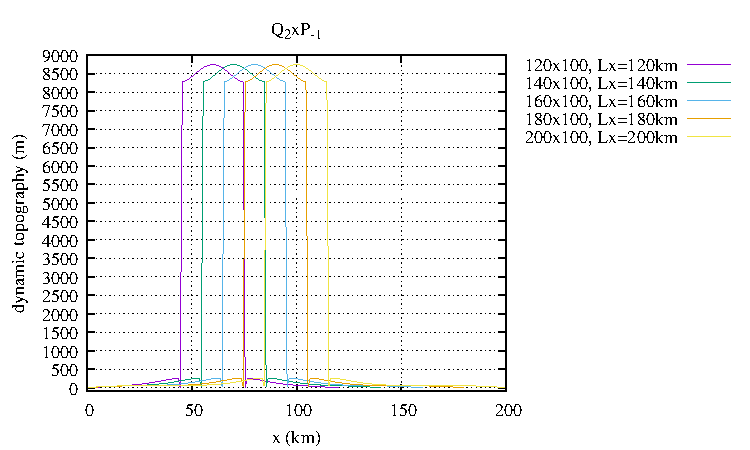
\includegraphics[width=8.5cm]{python_codes/fieldstone_160/results/dyn_topo6b.pdf}\\
{\captionfont Left: raw signal; Right: signal offset so that DT is zero on the 
sides of the domain.}
\end{center}
When looking at the raw signal, we find that the dynamic topography is less dependent on horizontal extent than before
but still increases by about 1000m.
However, we also must consider the negative topography on each side of the block. 
When offseting the topography signal so that it is zero on the sides of the domain (right figure)
we find that the DT is constant across the range of $L_x$ values!

 
In light of all this, I am a bit lost as to what this theoretical value 
stands for. I guess an infinitely long and deep domain? 
My plan is to revisit this with \aspect asap to make sure that these results are correct.


